%Linea Para poder completar automaticamente las citas con el Sublime
%No hace el documento, se puede borrar esta linea si no se usa el Sublime
%------------------------------------------------------------------------------
 \newcommand{\NoBiblioMicro}[1]{
 \ifthenelse{\equal{#1}{verdadero}}{}{\bibliography{Referencias/base_bibliografica}}
 \NoBiblioMicro{verdadero}}
 %-----------------------------------------------------------------------------

%Formato (Nombre de capitulo largo o corto), nombre del capitulo, resumen y estilo de la
%Portada del Capitulo
%------------------------------------------------------------------------------
 
 %Formato en si, titulo en dos renglones
 \FormatoCapituloDosLineas
 
 %Nombre y etiquete para referir
 \chapter{Microfabricación de los electrodos}\label{chap:Microfabricacion}

 %Para que no salga el numero de pagina en la portada del capitulo
 \thispagestyle{empty}
	
 %Resumen del Capitulo en Italica
 \noindent\textit{En este capitulo se describen los resultados obtenidos durante en la fabricación de electrodos cubiertos con películas delgadas mesoporosas de sílice. Se analizan los diseños utilizados, los materiales empleados, las técnicas aplicadas y las caracterizaciones llevadas a cabo. Principalmente se evaluó el desempeño electroquímico de los electrodos por un lado, y la compatibilidad con las síntesis sol-gel por otro, de forma de compatibilizar los procesos \textit{top-down }con los \textit{bottom-up.}}\index{bottom-up@\textit{bottom-up}}\index{top-down@\textit{top-down}}
 
 
 %Indice de capitulo alineada al borde inferior de la pagina, nueva pagina
 \vfill
 \minitoc
 \newpage
 %-------------------------------------------------------------------------------

\section{Introducción}
	
	El diseño y desarrollo de un multisensor electroquímico selectivo, integrado y escalable basado en \pdm\space consta de dos bloques constructivos fundamentales, las películas delgadas mesoporosas y los electrodos. En el capítulo \ref{chap:Mesoporosos}, se discutió y analizó la elección de los materiales para conformar la película delgada mesoporososa con la cual se recubren los electrodos. En el capítulo \ref{chap:Electroquimica} se realizó un estudio profundo sobre sus propiedades de transporte, la capacidad de preconcentrar, excluir, estabilidad química, etc.

	La integración de los procesos \textit{bottom-up}, propios de procesos de síntesis químicas, y \textit{top-down}, aquellos usados en microfabricación, no siempre es trivial. El sólo hecho de depositar soles con precursores de óxidos sobre oro, que resulten en películas delgadas homogéneas, bien adheridas sin grietas ni fisuras, ya es un desafío. El objetivo, luego de desarrollar los métodos a bajas temperaturas para la síntesis de \pdm, de optimizar y estudiar su estructura y de comprender los procesos de transporte a través de las películas, es poder depositarlos sobre estructuras de oro con un diseño optimizado para usarlo como sensor. 

	El depósito de soles sobre una superficie que tenga dos o más capas de distintos  materiales trae asociadas dificultades inherentes a las propiedades físicas y químicas de cada uno de ellas. Pueden diferir en el coeficiente de expansión térmica, en suquímica superficial, en su afinidad por el H$_2$O o solventes, etc.
	Es por ello que el diseño debe considerar los materiales que se usarán y sus propiedades, así como racionalizar la estructura de los electrodos considerando resistencia eléctrica, espesor de los electrodos y facilidad para la fabricación. También es fundamental tener en cuenta una serie de factores a la hora de mandar a imprimir las máscaras para los sensores. Principalmente la resolución de línea que se puede obtener según el tipo de máscara, cantidad de electrodos de trabajo por sensor, calcular el área óptima para obtener señales aceptables, estimar resistencias, distancias entre electrodos y demás parámetros.

	El material para los electrodos también se debe elegir cuidadosamente. Se trata de un compromiso entre tres factores; las dificultades para compatibilizar con óxido de las películas mesoporosas; obtener un respuesta electroquímica de calidad y, por último la facilidad para depositarlos y transferir diseños por litografía.

	En este trabajo se priorizó generar diseños compactos, miniaturizar los electrodos y optimizarlos para obtener respuestas electroquímicas de buen desempeño. El oro posee excelentes propiedades para llevar a cabo reacciones de oxido-reducción y obtener una respuestas confiables y repetibles. Si bien, el Au es el material óptimo para este tipo de mediciones, existen otros mas económicos y, en algunos casos mas fáciles de depositar (tintas de carbono, óxido de indio/estaño, carbono vitreo, etc.), sin embargo, su respuesta electroquímica es poco repetible, su rugosidades es muy variable y tienen grandes desviaciones de la idealidad (sobre todo a altas velocidades de barrido).\cite{Wi2000,Villullas2000}

	En este capítulo se presentan los resultados colectados durante la fabricación de los microelectrodos. Se da cuenta de los diseño, se discuten las ventajas y desventajas de los procesos empleados y se pone énfasis en la compatibilidad con los métodos utilizados para el depósito y condensación de las \pdm\space realizados por procesos sol-gel. Se evalúa la calidad de la transferencia del diseño, las dimensiones, la respuesta electroquímica de los mismos y la posibilidad de escalar para producir sensores electroquímicos basados en películas delgadas mesoporosas en cantidad.


	%se decidió que para logra este fin, explorar las propiedades de las películas delgadas de óxidos mesoporosos descritas con anterioridad. Nos dedicamos, como primera aproximación, a depositar estas películas de óxido sobre otra película delgada, esta vez de Au, que a su vez está depositada sobre algún sustrato rígido y térmicamente estable como vidrio u silicio, de forma de obtener una estructura bicapa electrodo\textbar mesoporoso. 

 	%Muchos de los trabajos que figuran el la bibliografía utilizan técnicas de electroquímica como herramienta de caracterización para películas mesoporosas con múltiples propósitos; como inferir estructuras de poros, accesibilidad, deducir propiedades de transporte y estimar variables del sistema. En este trabajo se plantea el uso de la electroquímica, no solo como herramienta de caracterización de películas mesoporososas sino también como técnica analítica. Para lograr dicho objetivo se evaluó el desempeño electroquímico de los electrodos de Au así como la viabilidad de ser utilizados como sustrato para el depósito de película delgada mesoporosa. Dichas películas serán el elemento activo, que actúa como membrana selectiva de los analitos electroactivos a cuantificar. 
	
\section{Microfabricación de los sensores}
		
	 	 En las siguientes secciones se analiza el diseño de los sensores y se discuten los resultados de la fabricación de los electrodos. Se discuten, también, las técnicas de microfabricación empleadas y las caracterizaciones realizadas sobre los mismos. Por último, se analiza la compatibilidad con las técnicas sol-gel para utilizarse como sustratos de películas delgadas mesoporosas.

  		\subsection{Consideraciones sobre el diseño}

			 Desde un principio surgió la idea de fabricar una plataforma con múltiples electrodos. De forma de tener sensores, para múltiples analitos, compactos y escalables. Para ello es importante hacer un diseño que tenga en cuenta los procesos que se usan en la industria electrónica, de forma de poder escalar el prototipo. Las siguientes secciones tratan esta temática; de que forma se pueden generar diseños de electrodos para un sensor multianalito y que procesos pueden llevarse a cabo de forma de escalarlos y compatibilizar con los procesos de síntesis sol-gel.

		 \subsubsection{Primer diseño}

		     El primer diseño contempló un sensor con cuatro electrodos de trabajo (ET) y preveía utilizar contraelectrodo (CE) y electrodo de referencia (ER) externos. 

		    	\begin{figure}[th!]
		 	       	\includegraphics[width=\textwidth]{Imagenes/diseno_mascara_v1.pdf}
 		       		\caption[Primer diseño y máscara de los sensores]{Diseño y máscara para la primera versión de los electrodos. A) diseño completo con 32 sensores de 4 ET cada uno, B) Detalles de las marcas de alineación, C) microscopía de la máscara ya impresa donde se ven las imperfecciones de la impresión.}
 		         	\label{fig:diseno_mascara_v1}
 		     		\end{figure}
 		 	 \pagebreak
 		     		
		      Se trabajó con dimensiones relativamente grandes, con dos geometrías distintas, electrodos circulares con un radio R=\SI{300}{\um} y electrodos cuadrados de lado L=\SI{500}{\um}. Éste primer diseño, aunque simple y con un aprovechamiento del espacio poco eficiente cuenta con algunas ventajas destacadas. Muy económico para la impresión de las máscaras, áreas grandes de electrodos y pistas (para poder colocar fácilmente puntas de prueba y obtener valores altos de intensidad de modo de familiarizarse con las primeras respuestas EQ) y sencillo de fabricar debido a las dimensiones utilizadas.
		      % . Esto diseño sirvió para familiarizarse con las primeras mediciones EQ y sencillo de fabricar.  
		
		      La figura \ref{fig:diseno_mascara_v1} muestra como fue este primer diseño. Se puede apreciar que la impresión de la máscara, no es exactamente igual al diseño, sino que se ve una deformación del mismo dada por la baja resolución de la impresora; estableciendo de esta forma limitaciones a la hora de diseñar con este tipo de máscaras. La contrapartida es el bajo costo de las mismas y la facilidad para obtenerlas en algunas librerías gráficas especializadas (el costo equivalente a una impresión de alta calidad sobre filminas de tamaño A4).
		
 		 \subsubsection{Segundo Diseño}

		 	 El segundo diseño, mas complejo y compacto, con un aprovechamiento espacial optimizado está compuesto por sensores cuadrados de \SI{1}{\cm} de lado. Cada uno tiene, a su vez, 6 ET circulares y dispuestos sobre una circunferencia imaginaria y equiangulares entre ellos (ver figura \ref{fig:mascara_diseno_v2} y {\ref{fig:diseno_mascara_v1}). Se hicieron seis tipos de sensores diferentes, variando el diámetro de los electrodos (con R=\SI{300}{\um}, \SI{200}{\um}, \SI{150}{\um},\SI{100}{\um} y \SI{20}{\um}). Además, este diseño, contempla la integración del CE y del ER en el mismo sensor. El CE se ubica en el centro del diseño y tiene un área 5 veces mayor a la de los ET para no limitar la velocidad de reacción respecto del ET \cite{Wi2000}. El ER se ubica rodeando el CE. Esta configuración de <<electrodos calesita>>, en donde los ET se encuentren equidistantes tanto del CE como del ER, asegura que los valores de resistencia, capacidad y los procesos difusivos sean equivalentes para cada electrodo.

		     %Mas adelante puedo colocar que se trata de un diseño flexible en el que puedo colcar mas electrodos calesita, 8 o 10 o 12
			     \begin{figure}[th!]
			 	    \begin{subfigure}[t]{0.395\textwidth}
			       	\includegraphics[width=\textwidth]{Imagenes/SistemaA.pdf}
			    	\end{subfigure}
					\begin{subfigure}[t]{0.595\textwidth}
			        \includegraphics[width=\textwidth]{Imagenes/diseno_3d.jpg}
			        \end{subfigure}
			     	\caption[Segundo diseño y máscara de los sensores]{Segundo diseño de los sensores. Izquierda: Diseño de un sensor con 6 electrodos de trabajo, contraelectrodo, electrodo de referencia y marcas de alineación. Derecha: Modelo en 3D para un sensor con celda electroquímica. En rojo los electrodos y en verde la resina que forma la celda, el espesor de la misma es de aproximadamente \SI{100}{\um} y puede contener un volumen aproximado de \SI{2}{\ul}.}
			     	\label{fig:mascara_diseno_v2}
			     	\end{figure}
	   
		     Para esta etapa se incluyeron dos máscaras más. Una segunda máscara que integra la celda electroquímica (realizada con una resina epoxi fotocurable, figura \ref{fig:mascara_su8}) en la oblea y una tercera para iluminar específicamente sobre el área de cada uno de los electrodos, con el objetivo de controlar reacciones químicas dentro de los poros, inducidas por luz UV, p. ej. activar un iniciador o controlar el grado de polimerización  (figura \ref{fig:mascara_funcionalizacion}).\cite{Andrieu-Brunsen2015,Herzog2015,Silies2015} Para ello se incluyeron marcas de alineación individuales en cada sensor. De esta forma se puede alinear cada uno con dicha máscara, incluso luego de cortar la oblea e individualizar los sensores. El detalle de este segundo juego de máscaras se muestra en la figura \ref{fig:impresion_diseno_V2}.
					\begin{figure}[th!]
			 	   	    \centering
			 	   	    \begin{subfigure}[t]{0.495\textwidth}
			        	\includegraphics[width=\textwidth]{Imagenes/mascara_revolver_electrodos.pdf}
			       		\caption{Máscara para la segunda versión de los electrodos, la cual contiene 46 sensores de \SI{1}{cm} de lado cada uno.}
			         	\label{fig:mascara_v2}
			     		\end{subfigure}
			     		\begin{subfigure}[t]{0.495\textwidth}
			     		\includegraphics[width=\textwidth]{Imagenes/impresion_mascaras_V2.pdf}
			    		\caption{Detalle del diseño de un sensor (A), marcas de alineación (B) y las imágenes de microscopías óptica de la máscara impresa (C) y (D).}
			    		\label{fig:impresion_diseno_v2_b}	
						\end{subfigure}
			     		\begin{subfigure}[t]{0.495\textwidth}
			         	\includegraphics[width=\textwidth]{Imagenes/mascara_revolver_celda.pdf}
			        	\caption{Máscara para depositar la fotorresina epoxi que dará lugar a la celda electroquímica.}
			         	\label{fig:mascara_su8}
			     		\end{subfigure}
						\begin{subfigure}[t]{0.495\textwidth}
			     		\includegraphics[width=\textwidth]{Imagenes/mascara_revolver_funcionalizacion.pdf}
			        	\caption{Máscara para iluminar específicamente sobre el área de cada uno de los electrodos de cada sensor.}
			         	\label{fig:mascara_funcionalizacion}
			     		\end{subfigure}
			     		\caption[Juego de máscara. Segunda versión]{Segunda versión de los sensores, (a) máscaras  para los electrodos, (b) detalle para un solo sensor, (c) máscara para las celdas, (d) máscara para la funcionalización.}
			     		\label{fig:impresion_diseno_V2}
			     	   	\end{figure}
	
		     En la figura \ref{fig:impresion_diseno_V2} se muestra el juego de mascaras completo usado para este segundo diseño y también una microscopía de la máscara ya impresa. Este segundo diseño, mejorado y con electrodos de menor tamaño, requirió una impresión de mejor calidad, lo cual se ve reflejado en la figura \ref{fig:impresion_diseno_v2_b} donde se ve que la impresión es fiel reflejo del diseño, incluso con detalles tan pequeños como cuadrados de \SI{10}{\um} de lado. 
			 %Para más detalles de la impresión consultar la sección \ref{sec:impresion_mascaras}, pág \pageref{sec:impresion_mascaras}.
				
 		\subsection{Transferencia de los diseños}

 			 Una vez revisado el diseño y con las máscaras impresas, se realizó la transferencia de los mismos por fotolitografía. Los fundamentos de la técnica ya fueron introducidos en la sección \ref{sec:intro_fotolito}, pág. \pageref{sec:intro_fotolito}.

 			 Se eligió una fotorresina de doble exposición (mas conocida en inglés como \textit{image-reversal}) por estar especialmente diseñada  para aplicaciones de decapado o \textit{lift-off}. Las variables de espesor resultante del proceso de \textit{spin-coating}, tiempo y temperatura de secado de solventes, tiempo de irradiación UV, tiempo y temperatura de curado y tiempo de revelado fueron tomados de los valores de referencia que figuran en la hoja de datos provista por el fabricante. \cite{TI35E} Los valores utilizados y detalles experimentales fueron expuestos en la sección \ref{sec:fotolito}, pág. \pageref{sec:fotolito}.

 			 Se recomienda, para esta fotorresina, que la relación de aspecto entre el ancho de linea y el espesor sea mayor a 2 ($L/e>2$), de forma de obtener paredes verticales y estructuras mecánicamente robustas. 

 				\begin{equation}
				\frac{L}{e} \geq 2, \hspace*{0.2cm}\text{con}\hspace{0.2cm}  e \approx \SI{3}{\um}		
 				\end{equation}

     		 A su vez se fijó una rotación tal (\SI{4000}{\minute}, velocidad final) que establezca un espesor de aproximadamente \SI{3}{\um} para que haya una discontinuidad en el deposito del metal entre las partes con y sin fotorresina, tal como muestra el esquema de la figura \ref{fig:undercut}.

					%Figura esquema undercutting
 				\begin{figure}[ht!]
 				\centering
 				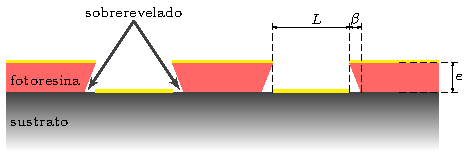
\includegraphics[width=0.75\textwidth]{Esquemas/altura-ancho.pdf}
 				\caption[Perfil de fotorresina para el decapado o\textit{ lift-off}]{Esquema de la fotoresina depositada y revelada, donde se muestra relación de espesor respecto del ancho de linea y el espacio para poder diluirla. El esquema muestra en particular un sobrerevelado aproximadamente del 20\%, para obtener buenos resultados durante el procesos de\textit{ lift-off}.}
 				\label{fig:undercut}
 				\end{figure}

 	   		 La variable más delicada, es, sin lugar a dudas, el tiempo de revelado, ya que es la que compensa los errores acumulados en el proceso. Cualquier irregularidad en el sistema de iluminación, inhomogeneidades en el espesor o calentamiento desparejo se ve reflejado en tiempos de revelado diferenciales para diferentes sectores. Dicho esto, mientras más grande el sustrato más difícil es lograr un revelado parejo. Es, también en este paso, donde se regula el <<sobrerevelado>> o, del inglés \textit{undercutting}, perfil necesario para que no se deposite metal en los laterales de la fotorresina, tal como se esquematiza en la figura \ref{fig:undercut}. El parámetro $\beta$ es la medida del sobrerevelado que es la diferencia entre la proyección en el sustrato de la superficie superior y la superficie inferior de la resina. Un $\beta \approx$\SI{500}{\nm} es el ideal para obtener buenos resultados en el procesos de \textit{lift-off}. 
 
 	         En la secuencia de imágenes de microscopia óptica de la figura \ref{fig:revelado} se muestra como evoluciona el revelado con el tiempo y, en particular, se ve en la última imagen de esta secuencia, el resultado final de la etapa de litografía y como el diseño resultó transferido de manera precisa.

 				%Imagnes revelado
 				\begin{figure}[th]
			 	   	    \centering
			 	   	    \begin{subfigure}[t]{0.235\textwidth}
			        	\includegraphics[width=\textwidth]{Imagenes/revelado1.jpg}
			       		\end{subfigure}
			     		\begin{subfigure}[t]{0.235\textwidth}
			     		\includegraphics[width=\textwidth]{Imagenes/revelado2.jpg}
			    		\end{subfigure}
			     		\begin{subfigure}[t]{0.235\textwidth}
			         	\includegraphics[width=\textwidth]{Imagenes/revelado3.jpg}
			        	\end{subfigure}
						\begin{subfigure}[t]{0.235\textwidth}
			     		\includegraphics[width=\textwidth]{Imagenes/revelado4.jpg}
			        	\end{subfigure}
			     		\caption[Revelado en función del tiempo]{Tiempos crecientes de revelado (de izquierda  a derecha (\SI{2.5}{min},\SI{3.5}{min},\SI{4.5}{min} y \SI{6}{min}) donde se aprecia como se disuelve la resina en la solución reveladora indicado por el cambio de color a medida que disminuye el espesor. Por último la oblea revelada por completo. Se deja un 20\% mas del tiempo necesario, para asegurarse un revelado total y para crear el perfil negativo de las paredes, especialmente útil para el proceso de\textit{ lift-off}.}
			     		\label{fig:revelado}
			     	   	\end{figure}

 		     Se llevó a cabo una segunda etapa de litografía (luego del deposito de Ti\textbar Au de para los electrodos) para colocar una resina fotocurable, epoxi, de alta viscosidad que genera estructuras de hasta \SI{100}{\um} de altura. En la fotografía de la figura \ref{fig:su8} se puede apreciar la alta viscosidad de la misma al momento de hacer el deposito por \textit{spincoating}. Nuevamente los datos para trabajarla se obtuvieron de la hoja de datos del fabricante\cite{Su8,Microchemicals2014} y los detalles experimentales fueron expuestos en  sección \ref{sec:fotolito}, pág. \pageref{sec:fotolito}. Esta resina se uso para hacer la celda electroquímica}, la cual puede contener un volumen aproximado \SI{2}{\ul} de solución. En las microscopias de la figura \ref{fig:resultados-su8} se muestra el resultado obtenido luego de alinear y depositar esta resina epoxi.

 				%Figura SU8 + alineacion + microscopia die con Su8
 				%Figura esquema undercutting
 				\begin{figure}[ht!]
 				\centering
 				\includegraphics[width=\textwidth]{Imagenes/SU8.jpg}
 				\caption[Deposito de la resina epoxi SU8]{Deposito por \textit{spin-coating }de la resina expoxi para encapsular. Se destaca la alta viscosidad de la misma, lo que permite formar paredes de hasta \SI{100}{\um} de espesor.}
 				\label{fig:su8}
 				\end{figure}

 				%Figura esquema undercutting
 				\begin{figure}[th]
			 	   	    \centering
			 	   	    \begin{subfigure}[t]{0.495\textwidth}
			        	\includegraphics[width=\textwidth]{Imagenes/alineacionSU8.pdf}
			       		\caption{Alineación de la segunda máscara con la pelicula de Ti\textbar Au ya depositada.}
			         	\label{fig:alineacion}
			     		\end{subfigure}
			     		\begin{subfigure}[t]{0.495\textwidth}
			     		\includegraphics[width=\textwidth]{Imagenes/DIE-SU8.pdf}
			    		\caption{Microscopía de uno de los sensores con la celda integrada.}
			     		\label{fig:die-su8}	
						\end{subfigure}
						\caption[Alineación y celda integrada en SU8]{Resultados de la alineación de la capa de los electrodos con la máscara para transferir la fotoresina epoxi (a) y, (b) detalle de un sensor terminado con celda EQ.}
			     		\label{fig:resultados-su8}
			     	   	\end{figure}

 		\subsection{Películas delgadas de Ti\textbar Au}

		 Como ya se mencionó anteriormente, los electrodos de los sensores son de Au y fueron depositados por la técnica de pulverización catódica o mas comúnmente conocida por su nombre en inglés \textit{sputtering}. La fabricación consistió primero en depositar una capa de al menos de \SI{20}{\nm} de espesor, llamada capa de  adherencia, la misma puede ser indistintamente de Ti o Cr, la cual promueve la adherencia del Au; sin esta capa el Au no adhiere sobre superficies no metálicas.\cite{Hieber1976} Una vez depositada la capa adherente y sin romper el vacío de la cámara del equipo, se depositaron \SI{150}{nm} de Au. El espesor resultó ser el óptimo para lograr un electrodo mecánicamente robusto y con buenas propiedades de conducción eléctrica pero suficientemente delgado para que las película delgadas mesoporosas sean continuas entre los electrodos y el sustrato. Para cada caso, en condiciones constantes, se puede realizar una curva de calibración. La misma se consigue graficando el espesor de las películas depositadas en función del tiempo, con el objetivo de establecer la tasa de depósito y así poder controlar el espesor de la película. 

		 Se optimizaron las condiciones de \textit{sputtering} para obtener películas homogéneas tanto en espesor como superficialmente. Para lograrlo se variaron los parámetros relevantes de la técnica, que son: la aceleración de los iones, determinada por diferencia de tensión entre el cátodo y ánodo; la densidad de corriente y el flujo de Ar. Una vez establecidas dichas condiciones se mantuvieron constante a lo largo de la tesis. El espesor de las películas metálicas, $d$, se reguló controlando el tiempo de depósito, $t$. De acuerdo a los los trabajos de Sigmund\cite{sigmund1968} y Seah\cite{Seah2005} éstas variables son directamente proporcionales según la ecuación \ref{eq:sputt}, donde $J$ es la densidad de corriente, $Y$ el rendimiento de la pulverización, $r$ el radio de los átomos de la muestra y $e_o$ la carga del electrón.

	 			\begin{equation}
	 				d=\left(\frac{JYr^3}{e_o}\right)t
	 				\label{eq:sputt}
	 			\end{equation}

		 Las condiciones de depósito de cada una de las sucesivas capas se detallan en la tabla \ref{tabla:sputt1}, pág. \pageref{tabla:sputt1}, para las películas metálicas y en la tabla  \ref{tabla:sputt2}, pág. \pageref{tabla:sputt2} para el SiO$_2$. 

		 		%figura FIB de los electrodos
						  \begin{figure}[ht!]
						  \begin{center}
						  \includegraphics[width=0.80\textwidth]{Imagenes/Perfil.jpg}
						  \caption[Sección trasversal de los eletrodos]{Corte transversal de los electrodos, donde se observan detalles de la bicapa Cr\textbar Au depositada sobre una oblea de silicio con un depósito aislante de SiO$_2$.}
						  \label{fig:FIB_electrodos}
						  \end{center}
						  \end{figure} 	

		 Para establecer las tasas de depósitos de cada una de la películas depositadas, se midió el espesor por diferentes técnicas. Para monocapas de Au y espesores pequeños típicamente menores a los \SI{30}{\nm}, se utilizó elipso espectrofotometría, los detalles experimentales y la base de la técnica ya fueron discutidos en la sección \ref{sec:elipso}, pág. \pageref{sec:elipso}. Para evaluar el apilamiento de sucesivas capas, inspeccionar la homogeneidad tanto en espesor como superficial, se utilizó microscopia electrónica de barrido (MEB) y haz focalizado de iones (FIB), técnica que permite hacer cortes e inspecciones de secciones transversales de los depósitos en distintos puntos. 

		 	%Grafico de la curva de calibración para el Au
					   		\begin{figure}[ht!]
					   		\begin{center}
							\includegraphics[width=0.75\textwidth]{Graficos/Espesor_Au.pdf}
							\caption[Curca de calibrado para el espesor de los electrodos]{Curva de calibración para establecer la tasa de de depósito de la capa de Au. La misma se realizó por pulverización catódica en las condiciones experimentales detalladas en la tabla \ref{tabla:sputt1}.}
							\label{fig:calibracionAu}
							\end{center}
							\end{figure}
		
		 En la figura \ref{fig:FIB_electrodos} se puede ver un corte transversal de los electrodos, realizado por FIB, donde se ven los espesores de ambas películas metálicas (Ti, capa adherente y Au), así como la capa dieléctrica de SiO$_2$. También se aprecia la buena homogeneidad en el espesor de cada una de las capas y en la superficie de la capa de Au, donde ocurrirá finalmente el intercambio electrónico entre las especies redox. Midiendo los espesores de las capas depositadas a distintos tiempos, podemos establecer la tasa de deposito, obtenida de la pendiente del figura \ref{fig:calibracionAu}. Como ya se mencionó en reiteradas ocasiones es de suma importancia conocer y controlar los espesores de cada una de las capas, ya sean películas delgadas mesoporosas, densas o metálicas.
		
  		\subsection{Decapado de la fotorresina o\textit{ lift-off}}

		 %En algun lugar se puede decir que se elijio lift-off en lugar de etching porque es mejor porque no se coloca fottoresina sobre los electrodos, etc, etc.

		 La última etapa de la fabricación de los electrodos, el decapado de la fotorresina, se conoce mas comúnmente con el nombre en inglés, \textit{lift-off} y consiste en disolver la fotorresina que queda como capa de sacrificio. En la figura \ref{fig:undercut} se pueden ver los sitios por donde da comienzo la disolución. La misma es completamente soluble en acetona. Cabe destacar, nuevamente, que es importante la disontinuidad de la película de oro para que tenga éxito esta etapa, ya que, si existe continuidad entre la parte que se quiere dejar y la que no, se generan imperfecciones en los bordes, o se desprende el metal de partes que no se desea. Para ello es muy importante saber bien los espesores que se logran durante el depósito, tanto de fotorresina como de película de Au, para regular la distancia que quede entre el metal en el sustrato y el metal sobre la resina; el esquema \ref{fig:undercut} presentado anteriormente en la pág. \pageref{fig:undercut} ejemplifica bien esta situación.

					  %Oblea Terminada V1
					  \begin{figure}[ht!]
					  \begin{center}
					  \includegraphics[width=\textwidth]{Imagenes/lift-off.jpg}
					  \caption[Proceso de decapado o\textit{ lift-off}]{Proceso de decapado o\textit{ lift-off}. Fotografía correpondiente a los electrodos del primer diseño, donde se muestra como a medida que se disuelve la fotorresina se va levantando el metal que esta sobre ella.}
					  \label{fig:ultrasonido}
					  \end{center}
					  \end{figure}

		 Por último, es importarte saber que es necesario aplicar ultrasonido; no alcanza con una simple inmersión de la oblea en solvente, hay que mantener una constante convección para la remoción de la fotorresina, que esta debajo del metal. A su vez, este proceso evita la redepositación del mismo sobre los electrodos (figura \ref{fig:ultrasonido}), ya que si ocurre este fenómeno es muy difícil, una vez que se seca la oblea, remover el metal de desperdicio pegado a los electrodos. Es en esta etapa final del proceso donde se demuestra si resultaron efectivas las etapas de limpieza y revelado. De haber algún residuo remanente durante la limpieza del sustrato o haber efectuado un revelado incompleto, llevará indefectiblemente a un desprendimiento de los electrodos del sustrato.

		 Finalmente, en las figuras \ref{fig:ObleaV1} y \ref{fig:ObleaV2}, se muestra el resultado final de la fabricación de los electrodos realizados en obleas de cuatro pulgadas (\SI{10}{\cm} de diámetro) para los dos diseños.

					  %Oblea Terminada V1
					  \begin{figure}[ht!]
					  \begin{center}
					  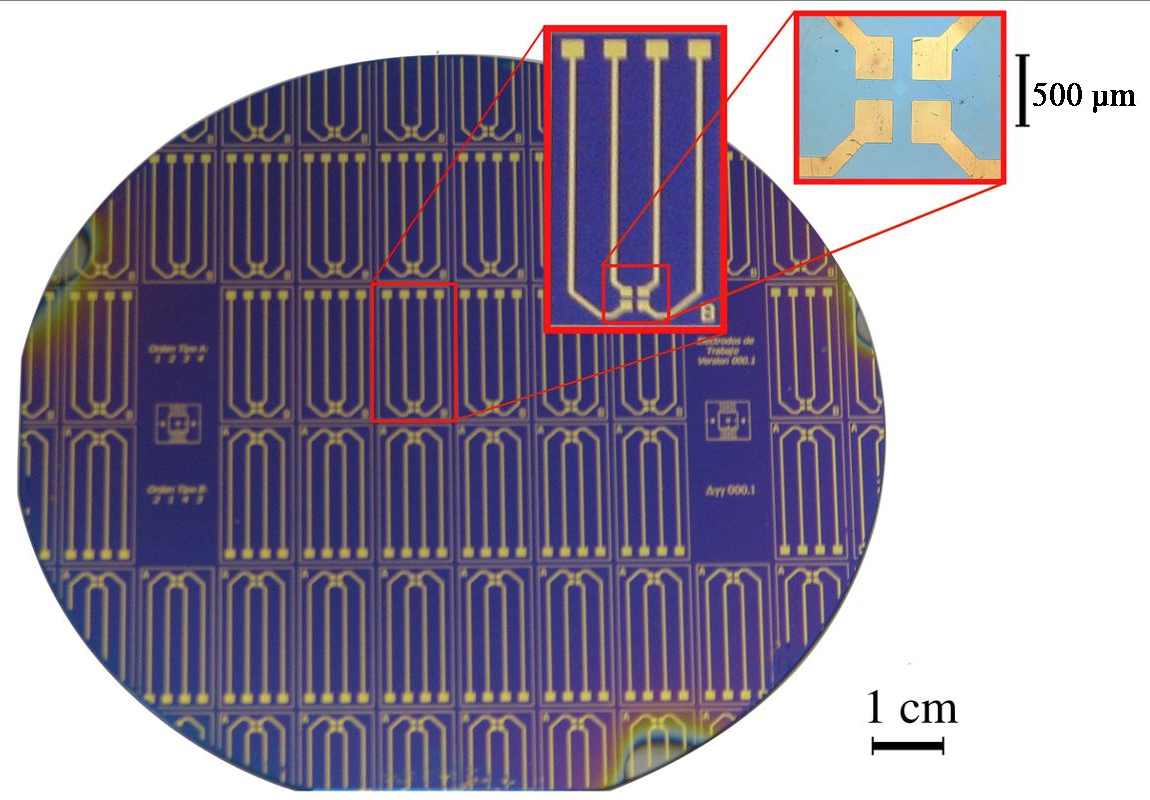
\includegraphics[width=\textwidth]{Imagenes/ObleaV1.jpg}
					  \caption[Electrodos, primera versión]{Primer diseño de los sensores. Oblea de silicio de \SI{10}{cm} de diámetro, capa de SiO$_2$ y 32 sensores con cuatro electrodos de trabajo cada uno.}
					  \label{fig:ObleaV1}
					  \end{center}
					  \end{figure} 	

					  %Oblea Terminada V2
					  \begin{figure}[ht!]
					  \begin{center}
					  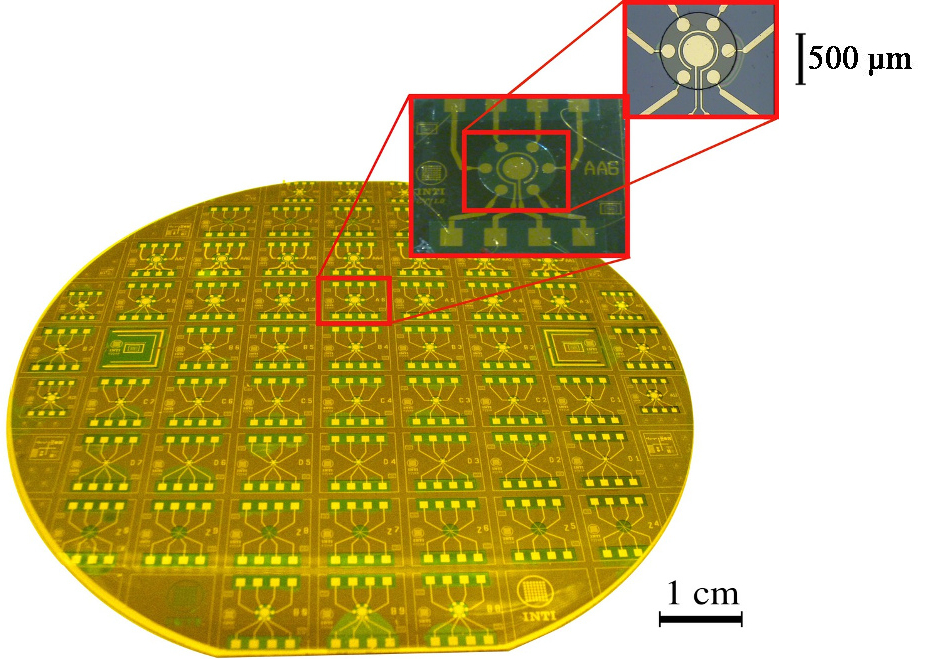
\includegraphics[width=\textwidth]{Imagenes/ObleaV2.jpg}
					  \caption[Electrodos, segunda versión]{Segundo diseño de los sensores. Oblea de silicio de \SI{10}{cm} de diámetro con 46 sensores con 6 electrodos de trabajo, contraelectrodo y pseudoreferencia. También se muestra la celda electroquímica depositada con resina epoxi SU-8.}
					  \label{fig:ObleaV2}
					  \end{center}
					  \end{figure} 	
		
\section{Caracterizaciones de los electrodos}

		Se dará cuanta en esta sección de las diferentes caracterizaciones y ensayos practicados sobre los electrodos de Au. Fundmentalmente la respuesta electroquímica, ya que la base de los sensores son las reacciones de oxido reducción. Es por ello que es necesario obtener electrodos de respuesta reproducible, confiable y fabricados por un proceso repetible y escalable. 

	\subsection{Respuesta electroquímica}\label{sec:respuesta_sondas_au}
			 		
			Una vez que los resultados de la fabricación de los sensores fueron óptimos se evaluó el desempeño electroquímico de los mismos. En el capítulo \ref{chap:Materiales} se describe con detalle el montaje experimental para realizar las mediciones de voltametrías cíclica (VC). Se usaron como sondas electroquímicas ferro y ferricianuro de potasio (\Ferro\space y \Ferri, \fe), cloruro de hexaaminorutenio(III) (\aminorutenioCompleto, \ru), hidroquinona (\hidroquinona, \hq) y ferroceno metanol \linebreak (\ferroceno, \fc). La elección de estas sondas modelos tiene que ver fundamentalmente con la carga neta de cada una de ellas, y con la reversibildiad de los pares redox. Analizaremos ahora como fue la respuesta de las películas delgadas de Au para cada una de estas sondas.
				
		\subsubsection*{Respuesta de ferro/ferricianuro de potasio}	 
			 	
		   En electroquímica este par redox es frecuentemente utilizado para evaluar la calidad de los electrodos, ya que es un par redox cuyas especies oxidada y reducida son económicas, fácil de conseguir, solubles en solución acuosa y se compartan de forma cuasireversible frente al intercambio electrónico electrodo-especie. La reacción que tiene lugar es la siguiente:
			 \begin{equation}
			 \schemestart 
			 Fe(CN)$_6^{4-}$  
			 \arrow{<=>[\scriptsize oxidación][\scriptsize reducción]}[0,1.5] 
			 Fe(CN)$_6^{3-}+e^-$ \schemestop
			 \end{equation}
		   Se espera, en la aproximación más simple, que sigan el comportamiento descrito por Randles-Sevcik, donde la intensidad de pico ($i_p$) es proporcional a la concentración ($C$) y a la velocidad de barrido a la $1/2$ $(v^{1/2})$ según:
		  
		 	\begin{equation}
			i_p=0.4463nFAC\left(\frac{nFvD}{RT}\right)^{1/2}
			\label{eq:rs2}
			\end{equation}

			\begin{figure}[ht]
	 	    	\begin{subfigure}[t]{0.5\textwidth}
	         	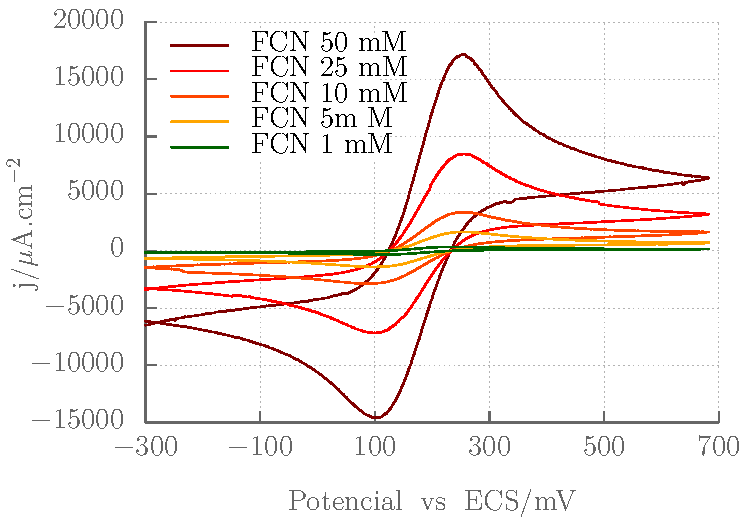
\includegraphics[width=\textwidth]{Graficos/Concentraciones_Fe.pdf}
	        	\caption{Voltametrías cíclicas para la cupla \fe\space a diferentes concentraciones. Todas medidas fueron tomadas a \SI{50}{\milli\volt\per\second}.}
	         	\label{fig:Fe_a}
	     		\end{subfigure}
     		 \begin{subfigure}[t]{0.495\textwidth}
	        	\includegraphics[width=\textwidth]{Graficos/Calibracion_Fe.pdf}
	       		\caption{Curva de calibración para distintas concentraciones de la cupla \fe\space valores tomados de la figura \ref{fig:Fe_a}.}
	         	\label{fig:Fe_b}
	     		\end{subfigure}
	     		%\vspace*{0.5cm}

 	     	\begin{subfigure}[t]{0.495\textwidth}
         		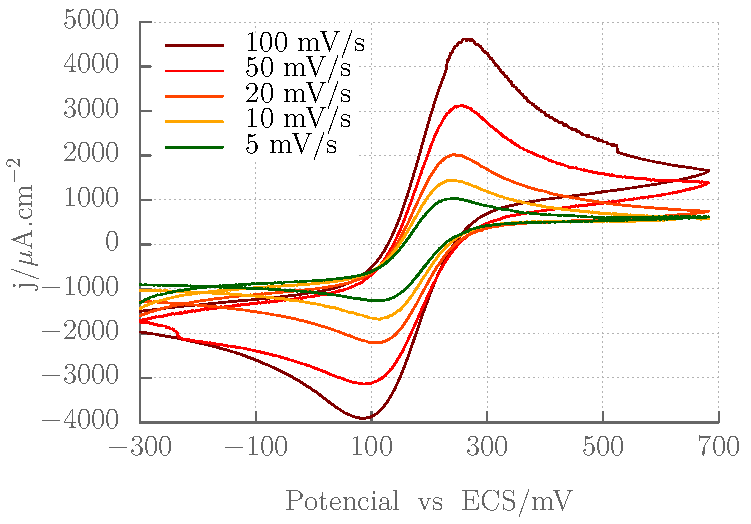
\includegraphics[width=\textwidth]{Graficos/Velocidades_Fe.pdf}
        	    \caption{Voltametrías cíclicas de una solución \SI{10}{\milli\Molar} de la cupla equimolar \fe\space a diferentes velocidades de barrido.}
        	    \label{fig:Fe_c}
     		 	\end{subfigure}
     	 	\begin{subfigure}[t]{0.495\textwidth}
        		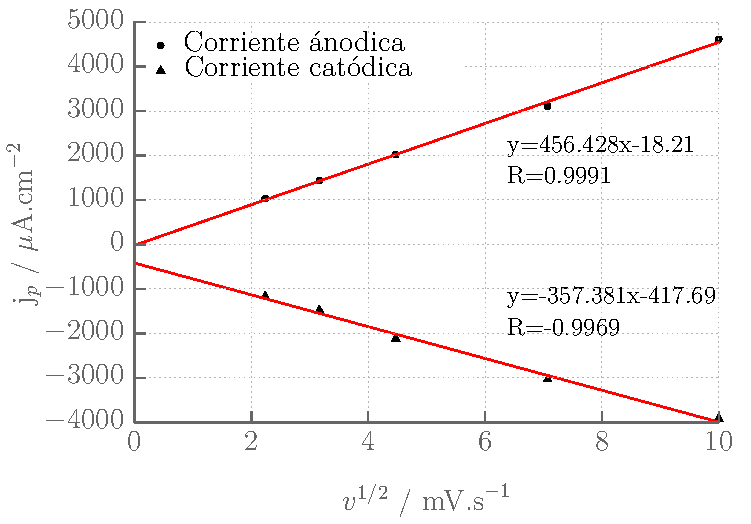
\includegraphics[width=\textwidth]{Graficos/VelocidadesCal_Fe.pdf}
       			\caption[Respuesta a diferentes velocidades de barrido para \fe]{Respuesta de la corriente de pico para \fe\space \SI{10}{\milli\Molar} frente a diferentes velocidades de barrido.}
         		\label{fig:Fe_d}
     			\end{subfigure}
     		 \caption[Respuesta electroquímica para \fe]{(a) Respuesta electroquímica de la cupla equimolar \fe\space para distintas concetraciones, (b) curva de calibrado para dichas concentraciones. (c) dependencia de la intensidad con la velocidad de barrido y, (d) dependencia lineal con la inversa de la raíz cuadrada de la velocidad de barrido. Todos los voltagramas fueron tomadas con contraelectrodo de Pt y en una solución 0,1M de NaCl como electrolito soporte, contra ESC.}
     		 \label{fig:ferro-ferri-CV}
     		 \end{figure}

     		 \pagebreak
		
		  	  Con el propósito de corroborar este comportamientos, se realizaron experimentos de VC a diferentes concentraciones de la sonda (figuras \ref{fig:Fe_a} y  \ref{fig:Fe_b}) y a distintas velocidades de barrido (figuras \ref{fig:Fe_c} y  \ref{fig:Fe_d}). Resultaron de especial utilidad la curva de calibración y la respuesta frente a distintas velocidades de barrido. Para cualquiera de estás velocidades los voltagramas conservan constantes los valores de $E^\circ$, indicativo de una buena trasferencia de carga entre el electrodo y la sonda. Además se destaca la relación del log(v) con el log(j$_p$), verificando la ecuación de Randles-Sevcik (ec. \ref{eq:rs2}).		  	  
  					
		  	  Con los resultados obtenidos para estas voltametrias se puede sugerir que el sistema responde a un proceso de difusión lineal semiinfinita, lo cual era lo que se esperaba en primer orden para un sistema en el que el electrodo esta embebido en solución con el analito electroactivo en solución de electrolito soporte {(\SI{0,1}{\milli\Molar} KCl, pH=$5.5$)\cite{Wi2000,Pumera2007,Gewirth2004,Villullas2000}.

	 	\subsubsection*{Respuesta del cloruro de hexaaminorutenio(III)}
	
	 	  Otra sonda electroquímica que se utilizó mucho y resultó relevante para este trabajo, es el cloruro de hexaaminorutenio(III). Esta molécula en solución se disocia para formar el complejo \aminorutenio. La reacción redox que tiene lugar es la siguiente:
	 		 	 	  		\begin{equation}
	 		 	 	 			\schemestart 
					 			 Ru(NH$_3$)$_6^{2+}$  
					 			 \arrow{<=>[\scriptsize oxidación][\scriptsize reducción]}[0,1.5] 
					 		 	 Ru(NH$_3$)$_6^{3+}+e^-$ \schemestop 
	 		 	 	 		\end{equation}
	 	  El intercambio entre los estados de oxidación Ru$^{3+}$/Ru$^{2+}$, responde a un proceso electroquímico reversible, en el cual podemos fácilmente reducir u oxidar el complejo variando el potencial del electrodo de trabajo. Habiendo ya comprobado, con el \fe, el buen desempeño de los electrodos respecto de la velocidad de barrido, se eligió un valor \SI{50}{\milli\volt\per\second} para las voltametrías cíclicas (de uso frecuente para este tipo de mediciones). Se llevaron a cabo una serie de VC para varias concentraciones de la sonda, con el objetivo de elaborar la correspondiente curva de calibración para \aminorutenio.
		
			 \begin{figure}[ht]
	 	     \begin{subfigure}[t]{0.495\textwidth}
	         	\includegraphics[width=\textwidth]{Graficos/Concentraciones_Ru.pdf}
	        	\caption{Voltametrías cíclicas para \ru\space a diferentes concentraciones.}
	         	\label{fig:Ru_a}
	     		\end{subfigure}
     		 \begin{subfigure}[t]{0.495\textwidth}
	        	\includegraphics[width=\textwidth]{Graficos/Calibracion_Ru.pdf}
	       		\caption{Curva de calibración para la especie \ru. Los valores fueron tomados de la figura \ref{fig:Ru_a}.}
	         	\label{fig:Ru_b}
	     		\end{subfigure}
	     		\label{rutenio}
	     		\caption[Respuesta electroquímica para \ru]{(a) Voltametrías cíclicas para soluciones de \ru\space de distinta concentración y, (b) curva de calibración para dichas concentraciones. Todos los voltagramas fueron tomados a \SI{50}{\milli\volt\per\second} con contraelectrodo de Pt en una solución \SI{0.1}{\milli\Molar} de NaCl contra ESC.}
	     	 \end{figure}
			 		 	 
		\subsubsection*{Respuesta del ferroceno metanol}
 	 	 
 	 	  El \fc\space fue otra de las sondas electroquímicas que se utilizó. A diferencia de las sondas anteriores la especie reducida de ésta molécula no tiene carga neta. Es por ello que resultó imprescindible para sacar conclusiones acerca de los fenómenos de transporte dentro las películas delgadas mesoporosas y sus propiedades permeoselectivas, como ya se discutió ampliamente en el capítulo anterior. La reacción de oxidación/reducción es la siguiente:
 	 	 			%Ecuación redox para el Ferroceno
 	 				 \begin{equation}
 	 	 				\begin{aligned}
 	 	 				\includegraphics[scale=0.75]{Esquemas/Redox-Fc.pdf}
 	 	 				\end{aligned}
 	 	 			 \end{equation}
 	 	  
 	 	 De la misma forma que se realizó para las otras sondas, se confeccionó una curva de calibración para distintas concentraciones de \fc\space, la \ref{Fig:Fc} muestra la respuesta electroquímica correspondiente sobre electrodos de Au.
 	 				
 	 				%Graficos para el Ferroceno
		 		 \begin{figure}[ht]
		 	      \begin{subfigure}[t]{0.495\textwidth}
		          	\includegraphics[width=\textwidth]{Graficos/Concentraciones_Fc.pdf}
		         	\caption{Voltametrías cíclicas para \fc\space a diferentes concentraciones, \SI{1}{\milli\Molar}, \SI{5}{\milli\Molar} y \SI{10}{\milli\Molar}.}
		          	\label{fig:Fc_a}
		      		\end{subfigure}
		      	 \begin{subfigure}[t]{0.495\textwidth}
		          	\includegraphics[width=\textwidth]{Graficos/Calibracion_Fc.pdf}
		         	\caption{Curva de calibración para la especie \fc. Los valores fueron tomados de la figura \ref{fig:Fc_a}.}
		          	\label{fig:Fc_b}
		      		\end{subfigure}
		      	 \caption[Respuesta electroquímica para \fc]{a) Voltametrías cíclicas para soluciones de \fc\space de distinta concetración y, b) curva de calibración para dichas concentraciones. Todos los voltagramas fueron tomadas a \SI{50}{\milli\volt\per\second} con contraelectrodo de Pt y en una solución \SI{0.1}{\Molar} de NaCl como electrolito soporte.}
		      	 \label{Fig:Fc}
	      		 \end{figure}

				% \subsubsection*{Respuesta de la hidroquinona}
				 	 
				%  	 	 La \hq\space a diferencia de las otras sondas que se utilizó durante la tesis, tiene dos características diferenciales; una es que tanto la forma oxidada como reducida no tienen carga neta (a lo largo de la tesis se desarrollará el concepto de sonda modelo cargada/neutra para demostrar la permeoselectividad de las membranas),  y la otra es que es el proceso de oxidación de la hidroquinona en benzoquinona, y su proceso inverso, de reducción nuevamente a hidroquinona, ambos son irreversibles. 

				%  	 	 La reacción redox que tiene lugar es la siguiente:
				 	 
				%  	 	  			%Ecuacion redox de la HQ
				%  	 	 				\begin{equation}
				%  	 	 				\begin{aligned}
				%  	 	 				\includegraphics[scale=0.75]{Esquemas/Redox-HQ.pdf}
				%  	 	 				\end{aligned}
				%  	 	 				\end{equation}
				%  	 	 			%Graficos para la HQ
				% 		 			\begin{figure}[ht]
				% 		 	     \begin{subfigure}[t]{0.495\textwidth}
				% 		         	\includegraphics[width=\textwidth]{Graficos/Concentraciones_HQ.pdf}
				% 		        	\caption{Voltametrías cíclicas para \hq\space a diferentes concentraciones, \SI{1}{\milli\Molar}, \SI{5}{\milli\Molar} y \SI{10}{\milli\Molar}.}
				% 		         	\label{fig:HQ_a}
				% 		     		\end{subfigure}
				% 	     		 \begin{subfigure}[t]{0.495\textwidth}
				% 		        	\includegraphics[width=\textwidth]{Graficos/Calibracion_HQ.pdf}
				% 		       		\caption{Curva de calibración para la especie \hq. Los valores fueron tomados de la figura \ref{fig:HQ_a}.}
				% 		         	\label{fig:HQ_b}
				% 		     		\end{subfigure}
				% 		     	 \caption[Respuesta electroquímica para \hq]{a) Voltametrías cíclicas para soluciones de \hq\space de distinta concetracionen y, b) curva de calibración para dichas concentraciones. Todos los voltagramas fueron tomadas a \SI{50}{\milli\volt\per\second} con contraelectrodo de Pt y en una solución \SI{0.1}{\Molar} de KCl como electrolito soporte.}
				% 	     		 \label{fig:HQ}
				% 	     		 \end{figure} 
				 
		 En la tabla \ref{tabla:sondas} se resumen las características y los resultados de las voltametrías cíclicas para cada una de las sondas modelo elegidas. Durante todo el desarrollo de la tesis se utilizaron estos resultados con ánimos de comparar las voltametrías sobre los electrodos desnudos y sobre los electrodos con la película mesoporosa.
		  %Tabla resultados EQ
		     \begin{table}[ht]
	  		  \caption{Resultados y características de las sondas electroactivas utilizadas.}
	  		  \begin{tabular}{>{\raggedright\arraybackslash}m{2.43cm}>{\centering\arraybackslash}m{3cm}>{\centering\arraybackslash}m{3cm}>{\centering\arraybackslash}m{2cm}}
	  		  \toprule
			  \multirow{2}{*}{Sonda}  	& Carga especie  & Carga especie  & \multirow{2}{*}{$\Delta$E(mV)} \\
			     		    & \hspace*{-0.79cm}reducida      & \hspace*{-0.85cm}oxidada  &	   \\ \midrule
	    	  \ferroferri	& \multirow{1}{*}{$4-$}  		& $3-$	     			   &  150  \\ \midrule
	  		  \aminorutenio & $2+$							& $3+$					   &  80   \\ \midrule
	  		  \raisebox{-.5\height}{\includegraphics[scale=0.5]{Esquemas/Fc.pdf}}   &  \hspace*{-0.29cm}0 & 1+ &  103  \\   		 
	  		  \bottomrule
	    	  \end{tabular}
	   		  \label{tabla:sondas}
			  \end{table}
		
			\pagebreak			

    \subsection{Incompatibilidad \textit{top-down/bottom-up}}

  			Una vez demostrado el buen desempeño electroquímico de los microelectrodos fabricados por técnicas \textit{top-down}, el siguiente paso fue el depósito de la película mesoporosa sobre los electrodos. Ya se discutió a lo largo del capítulo \ref{chap:Mesoporosos} las técnicas de deposito, el control sobre la síntesis para obtener películas de diferente porosidad, espesor, adherencia, etc.

  			Nos apoyamos en trabajos similares\cite{Otal2006,Calvo2009,Fattakhova-Rohlfing2007,Rohlfing2005}, donde utilizan la electroquímica como herramienta para establecer propiedades de las \pdm. En estos trabajos utilizan vidrio ITO o vidrio FTO como electrodos y desarrollan la electroquímica sobre sistemas más clásicos, películas delgadas calcinadas y electrodos no miniaturizados. En este trabajo, una vez depositadas las \pdm\space sobre los electrodos de oro, los resultados para \pdm\space calcinadas no fueron los esperados.  Mostraban, o voltametrias <<planas>>, o curvas donde la respuesta no era clara (figuras \ref{fig:Fe-Au-compa} y \ref{fig:Ru-Au-compa}). 

  			La búsqueda de la respuesta a este problema se encaró de forma sistemática. Partiendo de la hipótesis de que se trataba de algún contaminate, poros bloqueados o defectos durante la síntesis del mesoporosos, se repitió la preparación de los soles, los ensayos electroquímicos cambiando reactivos, sondas, solventes y electrolitos soportes. No pudiendo dar con la solución, se atribuyó el problema a alguna etapa de proceso. Se hicieron muestras control, donde se llevaron en paralelo los procesos de síntesis de películas mesoporosas, (descripto en la sección \ref{sec:cond_y_extr}, pág \pageref{sec:cond_y_extr}) pero sin la película. Es decir, sometiendo los electrodos de Au desnudos a condiciones de humedad y temperatura del proceso de síntesis de las \pdm. La respuesta electroquímica seguía siendo defectuosa, por lo que se planteó una nueva hipótesis. Esta nueva hipótesis, plantea que el problema de la mala respuesta EQ radica en someter los electrodos al tratamiento térmico de calcinación (\SI{350}{\celsius}).

  			Una vez que hallada la respuesta surgieron dos vías de acción, 1) Cambiar el material de los electrodos por oro de mayor calidad o platino, 2) sustituir o evitar el paso de calcinación. Se consideró la segunda opción mucho mas rica, tanto científica como tecnológicamente, ya que permitía resolver el problema y desarrollar un método de condensación y extracción para sintetizar películas delgadas mesoporosas de óxido de silicio. El desarrollo de este método alternativo ya fue extensamente tratado en el capítulo \ref{chap:Mesoporosos}.

  			Durante el desarrollo de los métodos alternativos de síntesis de \pdm\space se estudió, en paralelo, como afecta a los electrodos el tratamiento térmico, las resultados de las caracterizaciones se presentan a continuación.
			
		\subsubsection{Análisis de la superficie por XPS}

			Al surgir el problema luego del tratamiento térmico, se caracterizó la superficie en busca de interferencias , ya que trabajos anteriores demuestran que es posible la difusión, a la superficie del electrodo, de metales provenientes de la capa de adherencia \cite{Alonso1990,Moody2003}. Para ello, se analizó con espectroscopia de fotoelectrones emitidos por rayos X (XPS), la superficie del Au. Se depositaron dos electrodos de Cr\textbar Au sobre silicio, uno de ellos fue sometido a tratamiento térmico mientras que el otro no. Los resultados se muestran en el gráfico de la figura \ref{fig:XPS}, donde se evidenció la difusión hacia la superficie, de cromo ligado a oxigeno. Esto sugiere que el cromo, utilizado como capa de adherencia, se oxida y difunde cuando los sensores son sometido a una temperatura de \SI{350}{\celsius}.

				\begin{figure}[ht!]
		 	       	\begin{center}
		 	       	\includegraphics[width=0.85\textwidth]{Graficos/XPS.pdf}
		        	\caption[XPS de peliculas delgadas de Cr\textbar Au]{Espectroscopia de fotoelectrones emitidos por rayos (XPS) correspondiente a películas delgadas de Cr\textbar Au con (\usebox{\rojo}) y sin tratamiento térmico  (\usebox{\marron}). Observese los picos correspondiente al cromo y el aumento de la intensidad relativa del pico correpondiente al oxigeno, indicando la difución de Cr$_x$O$_y$ hacia la superficie de los electrodos.}
		         	\label{fig:XPS}
		         	\end{center}
		     		\end{figure}
		
		\subsubsection{Resistencia superficial}

			Una vez demostrada la difusión a través de las películas de Au, se midió la resistencia superficial, con el objetivo de corroborar algún cambio respecto en las propiedades eléctricas de los electrodos. Se midió la resistencia sobre 3 muestras, una sin tratamientos térmico, otra tratada a \SI{350}{\celsius} y la tercera tratada también a \SI{350}{\celsius} pero en atmósfera de vacío (\SI{e-5}{\milli\bar}) Los resultados se resumen en la tabla \ref{tabla:resistencia}, donde se corrobora que la resistencia por cuadrado es más alta en las muestras tratadas térmicamente, debido a la difusión de impurezas hacia la superficie. 

				\begin{table}[ht!]
			  		  \caption[Resistencia superficial de los electrodos]{Resistencia superficial de los electrodos con y sin tratamiento térmico.} 
			  		  \begin{tabular}{>{\raggedright\arraybackslash}m{4.2cm}>{\raggedright\arraybackslash}m{7.075cm}} 
			  		  \toprule
					  Muestra & Resistividad superficial $(\Omega/_{\square})$  \\ \midrule
			      	  Au \SI{350}{\celsius} 		  	& $3.720 \pm 0.001$		 \\	  
			      	  Au \SI{350}{\celsius} en vacío	& $3.685 \pm 0.001$		 \\	  
			      	  Au \SI{25}{\celsius}    	  		& $0.595 \pm 0.001$		 \\ 
			      	  \bottomrule
			    	  \end{tabular}
			    	  \label{tabla:resistencia}
			   		  \end{table}
		
		\subsubsection{Voltametrías cíclicas}

			La VC es una técnica analítica que tiene una respuesta que depende fuertemente de la superficie del electrodo.\cite{Wi2000,Pumera2007,Gewirth2004,Villullas2000} Con el propósito de comparar la respuesta de distintos metales para los electrodos, se tuvo la oportunidad de depositar electrodos de oro de mayor pureza, Au4N (99,99\% de \textit{Sigma Aldrich}) en lugar del Au3N (99,9\% de \textit{Eurometal}), el cual es mucho más económico, fácil de conseguir y es el blanco habitual para pulverización disponible en el laboratorio.  

			Se midieron por VC la respuesta de los electrodos Au3N calcinados y sin calcinar y se comparó con la obtenida para electrodos de Au de mayor (Au4N) pureza sometidos a calcinación. Los resultado de dichos experimentos se muestran en los voltagramas de las figuras \ref{fig:Fe-Au-compa} y \ref{fig:Ru-Au-compa} para \aminorutenio\space y \ferroferri\space respectivamente.

				\begin{figure}[ht]
		 	      \begin{subfigure}[t]{0.495\textwidth}
		          	\includegraphics[width=\textwidth]{Graficos/Fe-Au-Comparaciones.pdf}
		         	\caption{Voltametrías cíclicas para \fe\space \SI{1}{\milli\Molar} tomadas a \SI{50}{\milli\volt\per\second} en una solución \SI{0.1}{\Molar} de KCl.}
		          	\label{fig:Fe-Au-compa}
		      		\end{subfigure}
		      	 \begin{subfigure}[t]{0.495\textwidth}
		          	\includegraphics[width=\textwidth]{Graficos/Ru-Au-Comparaciones.pdf}
		         	\caption{Voltametrías cíclicas para \ru\space \SI{1}{\milli\Molar} tomadas a \SI{50}{\milli\volt\per\second} en una solución \SI{0.1}{\Molar} de KCl.}
		          	\label{fig:Ru-Au-compa}
		      		\end{subfigure}
		      	 \caption[Comparación entre electrodos calcinados y sin calcinar]{Voltametrías para \fe\space y \ru\space donde se compara la respuesta sobre electrodos de Au4N calcinado (\usebox{\oliva}) con electrodos de Au3N calcinado (\usebox{\negro}) y Au3N sin calcinar (\usebox{\rojo}). Se observa que la respuesta solo es afectada con los electrodos calcinados con Au3N.}
		      	 \label{Fig:Comparacion-Au}
	      		 \end{figure}	

			La primera observación que se desprende de los voltagramas es que la respuesta para el Au3N sin tratamiento térmico es prácticamente idéntica a la del Au4N con tratamiento térmico. Por otro lado la respuesta del oro menos purificado, Au3N, sometida a temperatura, muestra una clara irreversibilidad en los procesos de oxido reducción para ambas sondas, a tal punto que no se observa la reducción para \ferroferri\space (figura \ref{fig:Fe-Au-compa}, curva roja). Con estos resultados y lo expuesto anteriormente, queda claro que la respuesta anómala es debida a una capa superficial, generada por un proceso difusivo durante el tratamiento térmico. Este hecho dificulta la transferencia electrónica entre sonda-electrodo, alejándose de la idealidad y generando una separación de potenciales entre picos anódico y catódica. Como consecuencia directa se obtiene una respuesta EQ deficiente y no reproducible.  
			
    	\subsubsection{Microscopía electrónica de barrido}
			  		
			 En las microscopía de la figura \ref{fig:Au_compTT} se comparan depósitos de Au tratados térmicamente con depósitos no tratados. Se observa un crecimiento en el tamaño de partícula para los tratados térmicamente, a \SI{350}{\celsius}, temperatura para la vía clásica de síntesis de \pdm. Este hecho demuestra que esta temperatura es suficiente, para, al menos, producir un aumento en el tamaño de los cristales de las películas delgadas de oro. Dicha transformación también fue reportada a una temperatura menor, de \SI{300}{\celsius} por \v{S}vor\v{c}\'ik y colaboradores.}\cite{Svorcik2010}. Nuevamente nos encontramos con evidencia de transformaciones que sufren los electrodos al ser sometidos a un tratamiento térmico luego de ser depositado por pulverización catódica.

			 		\begin{figure}[th]
		 	   	    \begin{subfigure}[t]{0.49\textwidth}
			       	\includegraphics[width=\textwidth]{Imagenes/Au-sinTT.jpg}
			   		\end{subfigure}
			   		\begin{subfigure}[t]{0.49\textwidth}
			   	    \includegraphics[width=\textwidth]{Imagenes/Au-conTT.jpg}
			   		\end{subfigure}
					 \caption[Microscopía comparativa electrodos Au]{Microscopías de barrido electrónico donde se comparan los electrodos sin someter a tratamiento térmico (izquierda) con los sometido tratamientos térmico (derecha). Se observa un cambio en el tamaño de las partículas que forman los electrodos.}
					 \label{fig:Au_compTT}	
				     \end{figure}
		 		 		
		%\subsection{Comparación entre electrodos}

		     % 	%Compracion AU desnudo, Au INTI calcinado>

		     % 	Como etapa final de la optimización y caracterización de los sensores, se depositaron \pdm, sobre electrodos de Au de alta pureza calcinado (Au4N), y sobre electrodos de Au de baja pureza (Au3N) realizados a baja temperatura con el método de alto vacío (consultar \ref{sec:trat-vacio}, pág. \pageref{sec:trat-vacio} para más detalle). 

		     % 			 \begin{figure}[ht!]
				 	%       \begin{subfigure}[t]{0.495\textwidth}
				  %         	\includegraphics[width=\textwidth]{Graficos/Ru-F127-CNEA-Calcinado-0-1.pdf}
				  %        	\caption{Ciclos de VC para \ru\space \SI{0.1}{\milli\Molar} sobre un electrodo de Au4N calcinado, tomadas a \SI{50}{\milli\volt\per\second} en una solución \SI{0.1}{\Molar} de KCl.}
				  %         	\label{fig:Au4N-Ru1mM}
				  %     		\end{subfigure}
				  %     	 \begin{subfigure}[t]{0.495\textwidth}
				  %         	\includegraphics[width=\textwidth]{Graficos/Ru-F127-INTI-BajaT-0-1.pdf}
				  %        	\caption{Ciclos de VC para \ru\space \SI{0.1}{\milli\Molar} sobre un electrodo de Au3N sin calcinar, tomadas a \SI{50}{\milli\volt\per\second} en una solución \SI{0.1}{\Molar} de KCl.}
				  %         	\label{fig:Au3N-Ru1mM}
				  %     		\end{subfigure}
				  %     	 \caption[Comparación \pdm\space sobre diferentes electrodos]{Voltametrías cíclicas donde se compara el comportamiento de un electrodo de Cr\textbar Au de alta pureza sometidos a \SI{350}{\celsius} (a) con otro de baja pureza sin tratamiento térmico ambos recubiertos con una película delga mesoporosa de óxido de silicio (b).}
				  %     	 \label{fig:Comparacion-meso}
			  %    		 \end{figure}
			    
			  %  Estos experimentos tiene como motivación comparar y validar dos parámetros simultáneamente; por un lado la respuesta de electrodos de Au de alta pureza contra electrodos de Au de baja pureza y, por el otro, el comportamiento de las películas mesoporosas sintetizadas por el método clásico de calcinación, con aquellas sintetizadas con el método alternativo de vacío, desarrollado en esta misma tesis y cuyos resultados se expusieron en el capitulo \ref{chap:Optimizacion}.
		      % 	Los resultados fueron satisfactorios, tal como se muestran en las figuras \ref{fig:Au4N-Ru1mM} y \ref{fig:Au3N-Ru1mM}, donde se ve una respuesta prácticamente idéntica tanto para el sistema calcinado como para el sistema de baja temperatura. 
		      % 	Tanto la forma de Las diferencias que se observadas se discutirán en el próximo capitulo ya que tienen que ver con el trasporte y el modelo planteado para las difusión de sondas dentro de las películas porosa y no, con la naturaleza de la película de Cr\textbar Au.


			  % En la figura \ref{} se compara la voltametría, para \aminorutenio\space sobre un electrodo de Au3N y sobre otro recubierto con mesoporoso. Se ve allí, para el electrodo desnudo, que tanto la intensidad como la separación en potencial entre los picos catódicos y anódicos, muestran un proceso mucho mas irreversible de lo esperado para esta sonda, indicador de algún problema en la trasferencia electrónica entre analito y electrodo. La respuesta con el mesoporoso depositado es similar, con la diferencia que aquí se muestra como este ingresa en la película, la explicación detallada de este tipo de voltagrama se trata a fondo en el siguiente capítulo. Este resultado fue otro de los indicadores de que la película mesoporosa no es el problema, sino el electrodo.

			  % Aca va el cambio de au vs tratamientos de bajas temperaturas y aplicable a nuevos sustratos y por supuesto mucho mas economico (por el Au).

\section{Más allá de la microfabración}
	
	  Esta sección tiene por motivación mostrar y ejemplificar muy brevemente algunos experimentos, reflexiones y pruebas de concepto derivadas del presente trabajo. Estos experimentos generan nuevas incógnitas y abren lineas de investigación y desarrollo en el área sensores. No es el propósito de este apartado realizar demostraciones formales o hacer discusiones profundas de los resultados, sino mostrar los avances y conceptos surgidos durante esta tesis con perspectivas a futuros desarrollos e investigaciones.

	\subsection{Integración en microchips de silicio}

	  La ventaja de fabricar lectrodos por técnicas de microelectrónica es indiscutible. Hay muchas fabricas a nivel global  de microsistemas (MEMS) y circuitos integrados (IC) (conocidas en ingles simplemente como \textit{foundry}). Dichas fabricadas elaboran sus productos con procesos estándar de fabricación, por cada nodo tecnológico, con reglas de diseño claras y bien establecidas. La integración de sensores en circuitos integrados no es algo nuevo, y, dado el nivel de integración de la electrónica de las últimas décadas, es algo que siempre se debe detener en cuenta en la etapa de prototipado de sensores.\cite{Wang2012,Liu1993,Novell2012,Yu2013,Sarkar2014} Debido al desarrollo y optimización de los procesos para depositar \pdm\space a bajas temperaturas se podría fácilmente integrar los sensores EQ en solo chip con potenciostato integrado en la lógica del IC.
 	
 	\subsection{Sensores y electrodos flexibles e impresos}

 	  Se realizaron, durante este trabajo, pruebas conceptuales sobre impresión de mesoporosos. El objetivo fue transferir un diseño arbitrario sobre diversos sustratos, además, de esta forma se podrían imprimir \pdm\space de igual o distintos óxidos. Se trabajó en colaboración con el grupo del Dr. Baumann, del \textit{Department of Digital Printing and Imaging Technology} de la \textit{Technische Universität Chemnitz} de Alemania (\url{https://www.tu-chemnitz.de/mb/DigiTech/professorship.php}). Allí se realizaron pruebas de concepto imprimiendo soles modificados con etilenglicol con un equipo de inyección de tinta sobre diversos soportes. Los procesos a baja temperatura desarrollos en este trabajo, no solo hacen que disminuya la difusión entre las capas metálicas, permitiendo la integración en chips de silicio, sino que permite depositar las \pdm\space sobre sustratos térmicamente menos estables. Los resultados fueron sistemas porosos de soles de SiO$_2$, estructurados con F127 impresos sobre silicio, oro, microelectrodos y poliestireno de alto impacto (PAI). Se muestran, en la figura \ref{fig:flexibles}, patrones cuadrados impresos sobre una diversidad de sustratos variando, con el objetivo de encontrar las condiciones óptimas para su impresión.

 		%imagenes Meso en Au, Meso en Silicio, Meso en Au con patrones, SEM
 	  		\begin{figure}[th]
			 	   	    \centering
			 	   	    \begin{subfigure}[t]{0.495\textwidth}
			        	\includegraphics[width=\textwidth]{Imagenes/Inkjet-02-escala-fondo.jpg}
			        	\caption{\pdmF\space impresos sobre oblea de silicio.}
			       		\end{subfigure}
			     		\centering
			     		\begin{subfigure}[t]{0.495\textwidth}
			     		\includegraphics[width=0.85\textwidth]{Imagenes/Inkjet-05-escala-fondo.jpg}
			    		\caption{\pdmF\space impresos sobre oblea de silicio con un depósito de Ti\textbar Au.}
			    		\end{subfigure}
			    		\centering
			    		\begin{subfigure}[t]{0.495\textwidth}
			         	\includegraphics[width=0.80\textwidth]{Imagenes/Inkjet-04-escala-fondo.jpg}
			        	\caption{\pdmF\space impresos sobre microelectrodos.}
			        	\end{subfigure}
			        	\centering
			        	\begin{subfigure}[t]{0.495\textwidth}
			     		\includegraphics[width=\textwidth]{Imagenes/Inkjet-03-escala-fondo.jpg}
 			        	\caption{\pdmF\space impresos en Ti\textbar	Au en soporte de poliestireno de alto impacto.}
			        	\end{subfigure}
			     		\caption[Electrodos impresos]{Fotografías de patrones impresos de óxido de silicio mesoporoso por inyección de tinta. Los poros fueron moldeados con F127 y la condensación se realizó por el método de alto vacío. La extracción se llevó a cabo con 2-propanol y agua.}
			     		\label{fig:flexibles}
			     	   	\end{figure}
			     	  
 	  Con la expectativa de poder realizar todo el proceso de fabricación de los sensores con técnicas de impresión, se muestran en la figura \ref{fig:tintas}, electrodos impresos por inyección con tintas a base a nanotubos de carbono desarrolladas en el INTI-CMNB. Actualmente estas tintas están en desarrollo y en proceso de optimización para uso en sensores EQ y enzimáticos\cite{Longinotti2010,Mass2016}. En la figura \ref{fig:tintas} también se muestra la respuesta EQ para \fe\space \SI{2.5}{\nm}, si bien no es la misma que en electrodos de Au, es una respuesta reproducible y confiable. Se prevé próximamente imprimir ambos componentes en un solo sustrato, los electrodos y películas delgadas mesoporosos.

 	  	%imagenes flexo + voltagrama
 	  			\begin{figure}[th]
		 	   	    \begin{subfigure}[t]{0.25\textwidth}
			       	\includegraphics[width=\textwidth]{Imagenes/NTC1-fondo.jpg}
			   		\end{subfigure}
			   		\begin{subfigure}[t]{0.25\textwidth}
			       	\includegraphics[width=\textwidth]{Imagenes/NTC2-fondo.jpg}
			   		\end{subfigure}
			   		\begin{subfigure}[t]{0.43\textwidth}
			   	    \includegraphics[width=\textwidth]{Graficos/TintaNTC-FeCN2-5mM.pdf}
			   		\end{subfigure}
					 \caption[Electrodos de NTC flexibles.]{Electrodos impresos por inyección de tinta en base a nanotubos de carbono donde se muestra la flexibilidad de la tinta y su respuesta electroquímica con una sonda de \fe\space \SI{2.5}{\milli\Molar} en solución de KCl \SI{100}{\milli\Molar}}
					 \label{fig:tintas}	
				     \end{figure}
 		

\section{Conclusiones parciales}

	A lo largo de este capítulo se presentan los resultados obtenidos durante el proceso de fabricación de los microelectrodos. Se hicieron dos diseños, de los cuales el segundo (retroalimentado de la experiencia del primero) es mas compacto, incorpora mas electrodos por sensor y prevé el uso de contraeletrodo y referencia integrados en el mismo.
	
	Los mismos fueron fabricados por un conjunto de técnicas conocidas como \textit{top-down}, propios de la microelectrónica. Fotolitografía óptica, deposición por pulverización catódica y \textit{lift-off}, entre otras. Encontradas las condiciones óptimas de proceso para cada etapa, y, conforme con los resultados, se evaluó el desempeño electroquímica de los mismos, la cual resulto ser muy satisfactoria. La siguiente etapa fue la de colocar la \pdm\space sobre ellos, discutida extensamente en el capítulo \ref{chap:Mesoporosos}. En esta etapa surgieron algunas dificultades,en particular, en lo referente al sensado electroquímico, pudimos detectar fenómenos de difusión hacia la superficie del electrodo durante la calcinación de las películas de SiO$_2$ mesoporosa sobre ellos, impidiendo el intercambio de electrones sonda-electrodo. 

	Este fue uno de los motores (junto con con otros como utilizar polímeros, evitar calcinaciones y reducir costos) para el desarrollo de procesos de síntesis de películas mesoporosas de SiO$_2$, a temperaturas menores que las clásicas de calcinación, donde se minimizan los procesos difusivos y no es necesario recurrir a material de ultra pureza.

	Las consecuencias directas de este desarrollo fueron que se pudo continuar depositando los óxidos sobre Au metalúrgico (Au3N) sin perder desempeño analítico y, a su vez, permitió depositar las \pdm\space sobre sustratos que sean estables a \SI{130}{\celsius}. Esto permitió acceder a sustratos flexibles, económicos y poder utilizar otros materiales como electrodos. Es en está área donde se incursionó imprimiendo tintas basadas en nanotubos de carbo y peliculas delgadas me soporosas de óxido de silicio sobre diversa cantidad de sustratos, incorporando las \pdm\space como sensores EQ al campo de la electrónica

	